\documentclass[12pt]{article}
\usepackage[svgnames,x11names,table]{xcolor}
\usepackage{hyperref}
\usepackage{graphicx}
\usepackage{parskip}
\usepackage{float}
\usepackage{amsmath}
\usepackage{amssymb}
\usepackage{enumitem}
\usepackage[thicklines]{cancel}

\hypersetup{
    colorlinks,
    citecolor=blue,
    filecolor=black,
    linkcolor=black,
    urlcolor=RoyalBlue4,
}

\title{PEU 218 Assignment 2}
\author{Mohamed Hussien El-Deeb (201900052)}
\date{\today}

\begin{document}

\maketitle
\tableofcontents
\hypersetup{linkcolor=RoyalBlue4}

\newpage
\section{Question 1}

\subsection{Problem}

Evaluate
\[
    \int_C \left(2y x^2 - 4x\right) d r
\]

Where \(C\) is lower half of the circle centered at the origin of radius 3 with clockwise
rotation.

\subsection{Solution}

\[x = 3 \cos(\theta)\]

\[y = 3 \sin(\theta)\]

\[
    \vec{r} = \left\langle x, y\right\rangle =
    \left\langle 3 \cos(\theta), 3 \sin(\theta)\right\rangle
\]

\[
    d \vec{r} = 3 \left\langle -\sin(\theta), \cos(\theta)\right\rangle d\theta
\]

\[
    d r = 3 d \theta
\]



The limits of integration are \(\theta = \pi \) to \(\theta = 0\).

\[
    \int_C \left(2y x^2 - 4x\right) d r
    = 18 \int_{\pi}^{0} \left(9 \sin(\theta) \cos^2(\theta) - 2 \cos(\theta)\right) d \theta
\]

\[
    = 18 {\left[3 \cos^3(\theta) + 2 \sin(\theta)\right]}_{0}^{\pi}
    = -108
\]

\newpage
\section{Question 2}

\subsection{Problem}

Evaluate \(\int_C \vec{F} \cdot d \vec{r}\), where
\(\vec{F}=\left\langle y, 3y^3 - x, z\right\rangle \) and the path \(C\) is defined by
\(C(t) = \left\langle t, t^n, 0\right\rangle, 0 \leq t \leq 1\) where \(n = 1, 2, 3, .. \)

\subsection{Solution}

\[
    \vec{r} = \left\langle t, t^n, 0\right\rangle
\]

\[
    d \vec{r} = \left\langle 1, n t^{n - 1}, 0\right\rangle d t
\]

\[
    \vec{F} = \left\langle t^n, 3t^{3n} - t, 0\right\rangle
\]

\[
    \vec{F} \cdot d \vec{r} = 3 n t^{4n - 1} + (1 - n) t^n d t
\]

\[
    \int_{0}^{1} \left(3 n t^{4n - 1} + (1 - n) t^n\right) d t
\]

\[
    = {\left[\frac{3}{4} t^{4n} + \frac{1 - n}{1 + n} t^{n + 1}\right]}_{0}^{1}
    = \frac{3}{4} + \frac{1 - n}{1 + n}
\]

\newpage
\section{Question 3}

\subsection{Problem}

Evaluate \(\int_C \vec{F} \cdot d \vec{r}\), where \(\vec{F} = \langle xy, 1 + 3y, 0\rangle \) and
\(C\) is the line segment from \((0, -4)\) to \((-2, -4)\) followed by portion of \(y = -x^2\)
from \(x = -2\) to \(x = 2\) which is in turn followed by the line segment from \((2, -4)\)
to \((5, 1)\).

\subsection{Solution}

I will reduce the dimension of the problem to 2D since \(\vec{F}\) is the
only 3D vector and its z component is 0.

\begin{figure}[H]
    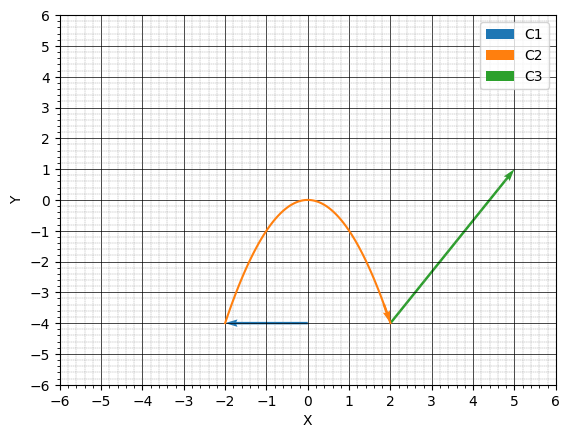
\includegraphics[width=\linewidth]{Q3.png}
    \caption{Path equations for the three contours.\cite{El-Deeb_PEU-218_Assignments_py}}\label{fig:Q3}
\end{figure}

\[
    \vec{F} = \left\langle xy, 1 + 3y\right\rangle
\]

\[
    C1 = \left\langle -2t, -4\right\rangle, \quad t = [0, 1]
\]

\[
    \vec{F}_1 = \left\langle 8t, -11 \right\rangle
\]

\[
    d \vec{r}_1 = \left\langle -2, 0\right\rangle d t
\]

\[
    C2 = \left\langle t, -t^2\right\rangle, \quad t = [-2, 2]
\]

\[
    \vec{F}_2 = \left\langle -t^3, 1 - 3t^2\right\rangle
\]

\[
    d \vec{r}_2 = \left\langle 1, -2t\right\rangle d t
\]

\[
    C3 = \left\langle 3t + 2, 5t -4\right\rangle, \quad t = [0, 1]
\]

\[
    \vec{F}_3 = \left\langle 15t^2 - 2t - 8, 15t - 11\right\rangle
\]

\[
    d \vec{r}_3 = \left\langle 3, 5\right\rangle d t
\]

\[
    \int_C \vec{F} \cdot d \vec{r}
    = \int_{C1} \vec{F}_1 \cdot d \vec{r}_1
    + \int_{C2} \vec{F}_2 \cdot d \vec{r}_2
    + \int_{C3} \vec{F}_3 \cdot d \vec{r}_3
\]

\[
    = \int_{-2}^{2} \left(5t^3 - 2t\right) d t
    + \int_{0}^{1} \left(45t^2 + 53t - 79\right) d t
\]

\[
    = \left[\frac{5}{4} t^4 - t^2\right]_{-2}^{2}
    + {\left[15t^3 + \frac{53}{2} t^2 - 79t\right]}_{0}^{1}
    = -37.5
\]

\newpage
\section{Question 4}

\subsection{Problem}

Evaluate \(\iint_S 2y\ dS\) where \(S\) is the portion \(y^2 + z^2 = 4\) between \(x = 0\)
and \(x = 3 - z\).

\subsection{Solution}

\[
    x = x, \quad y = 2\cos(\theta), \quad z = 2\sin(\theta)
\]

\[
    d\vec{S} = \frac{\partial \vec{r}}{\partial x} \times \frac{\partial \vec{r}}{\partial \theta}
\]

\[
    \vec{r} = \left\langle x, 2 \cos(\theta), 2 \sin(\theta)\right\rangle
\]

\[
    \frac{\partial \vec{r}}{\partial x} = \left\langle 1, 0, 0\right\rangle dx, \quad \frac{\partial \vec{r}}{\partial \theta} = 2 \left\langle 0, -\sin(\theta), \cos(\theta)\right\rangle d \theta
\]

\[
    \frac{\partial \vec{r}}{\partial x} \times \frac{\partial \vec{r}}{\partial \theta} = 2 \left\langle 0, \cos(\theta), \sin(\theta)\right\rangle d\theta dx
\]

\[
    dS
    = \left\lVert \frac{\partial \vec{r}}{\partial x} \times \frac{\partial \vec{r}}{\partial \theta} \right\rVert
    = 2 dx d\theta
\]

\[
    \iint_S 2y\ dS
    = 8 \int_{0}^{2\pi} \int_{0}^{3 - 2 \sin(\theta)} \cos(\theta) dx d\theta
\]

\[
    = 8 \int_{0}^{2\pi} \left[3 - 2 \sin(\theta)\right] \cos(\theta) d\theta
\]

\[
    = 8 \int_{0}^{2\pi} \left[3 \cos(\theta) - 2 \sin(\theta) \cos(\theta)\right] d\theta
\]

\[
    = 8 \left[3 \sin(\theta) + \cos^2(\theta)\right]_{0}^{2\pi}
    = 0
\]

\newpage
\section{Question 5}

\subsection{Problem}

Let the temperature of a point in space be given by \(T(x, y, z)= 3x^2 + 3z^2\).
Compute the heat flux across the surface \(x^2 + z^2 = 2, 0 \leq y \leq 2\), if \(k = 1\).
(Give a physical explanation to justify the sign of your result?)

\subsection{Solution}

The heat flux is given by \( -k \nabla T \).

\[
    - \iint_S \nabla T \cdot d\vec{S}
\]

\[
    \nabla T
    = \left\langle \frac{\partial T}{\partial x}, \frac{\partial T}{\partial y}, \frac{\partial T}{\partial z}\right\rangle
\]

\[
    = 6 \left\langle x, 0, z\right\rangle
\]

\[
    x = \sqrt{2} \cos(\theta), \quad y = y, \quad z = \sqrt{2} \sin(\theta)
\]

\[
    d\vec{S}
    = \frac{\partial \vec{r}}{\partial y} \times \frac{\partial \vec{r}}{\partial \theta}
\]

\[
    \vec{r} = \left\langle \sqrt{2} \cos(\theta), y, \sqrt{2} \sin(\theta)\right\rangle
\]

\[
    \frac{\partial \vec{r}}{\partial y}
    = \left\langle 0, 1, 0\right\rangle dy, \quad \frac{\partial \vec{r}}{\partial \theta}
    = \sqrt{2} \left\langle -\sin(\theta), 0, \cos(\theta)\right\rangle d\theta
\]

\[
    d\vec{S}
    = \frac{\partial \vec{r}}{\partial y} \times \frac{\partial \vec{r}}{\partial \theta}
    = \sqrt{2} \left\langle \cos(\theta), 0, \sin(\theta)\right\rangle dy d\theta
\]

\[
    \nabla T \cdot d\vec{S}
    = 12 \left\langle \cos(\theta), 0, \sin(\theta)\right\rangle \cdot \left\langle \cos(\theta), 0, \sin(\theta)\right\rangle dy d\theta
    = 12 dy d\theta
\]

\[
    -\iint_S \nabla T \cdot d\vec{S}
    = - 12 \int_{0}^{2\pi} \int_{0}^{2} dy d\theta
    = - 48 \pi
\]

The negative sign indicates that the heat is flowing into the surface. This is because heat moves
from higher temperature in this case outside since temperature increases as we get away radially
from x and z origin to lower temperature inside the surface.

\newpage
\section{Question 6}

\subsection{Problem}

Evaluate \(\iint_S \vec{F} \cdot d S\) where
\(\vec{F} = y \hat{\imath} + 2x \hat{\jmath} + (z - 8) \hat{k}\) and \(S\) is the surface of the
solid bounded by \(4x + 2y + z = 8, z = 0, y = 0\) and \(x = 0\) with the positive orientation.
Note that all four surfaces of the solid are included in \(S\).

\subsection{Solution}

\[
    \iint_S \vec{F} \cdot d S
    = \iint_{S_1} \vec{F} \cdot d S_1
    + \iint_{S_2} \vec{F} \cdot d S_2
    + \iint_{S_3} \vec{F} \cdot d S_3
    + \iint_{S_4} \vec{F} \cdot d S_4
\]

For \(x = 0\),

\[
    S_1: 4x + 2y + z = 8 \rightarrow z = 8 - 2y
\]

\[
    \iint_{S_1} \vec{F} \cdot d S_1 = \int_{0}^{4} \int_{0}^{8-2y} \left( \vec{F} \cdot \hat{\dot{\imath}} \right) dz dy
\]

\[
    = \int_{0}^{4} \int_{0}^{8-2y} y dz dy
    = \int_{0}^{4} y(8-2y) dy
    = \left\lbrack 4y^2 - \frac{2}{3}y^3 \right\rbrack_{0}^{4}
    = \frac{64}{3}
\]

For \(y = 0\),

\[
    S_2: 4x + 2y + z = 8 \rightarrow z = 8 - 4x
\]

\[
    \iint_{S_2} \vec{F} \cdot d S_2 = \int_{0}^{2} \int_{0}^{8-4x} \left( \vec{F} \cdot \hat{\dot{\jmath}} \right) dz dx
\]

\[
    = \int_{0}^{2} \int_{0}^{8-4x} 2x dz dx
    = \int_{0}^{2} 2x(8-4x) dx
    = \left\lbrack 8x^2 - \frac{4}{3}x^3 \right\rbrack_{0}^{2}
    = \frac{64}{3}
\]

For \(z = 0\),

\[
    S_3: 4x + 2y + z = 8 \rightarrow y = 4 - 2x
\]

\[
    \iint_{S_3} \vec{F} \cdot d S_3 = \int_{0}^{2} \int_{0}^{4-x} \left( \vec{F} \cdot \hat{k} \right) dy dx
\]

\[
    = -8 \int_{0}^{2} \int_{0}^{4-x} dy dx
    = -8 \int_{0}^{2} (4-x) dx
    = -8 \left\lbrack 4x - \frac{1}{2}x^2 \right\rbrack_{0}^{2}
    = -48
\]

for \(\hat{n} = \frac{1}{\sqrt{21}} \left\langle 4, 2, 1\right\rangle \),

\[
    \iint_{S_4} \vec{F} \cdot d S_4 = \iint_{S_4} \left( \vec{F} \cdot \hat{n} \right) \left\vert \nabla f \right\vert dx dy
\]

\[
    \iint_{S_4} \vec{F} \cdot d S_4 = \iint_{S_4} \left( 2 y \right) dx dy
\]

\[
    = \int_{0}^{-4} \int_{0}^{4 + y} 2y dx dy
    = \int_{0}^{-4} 2y(4 + y) dy
    = \frac{32}{3}
\]

\[
    \iint_S \vec{F} \cdot d S = \frac{64}{3} + \frac{64}{3} - 48 + \frac{32}{3}
    = \frac{16}{3}
\]

\newpage
\bibliographystyle{plain}
\bibliography{references}
\nocite{El-Deeb_PEU-218_Assignments}

\end{document}